\def\pgfsysdriver{pgfsys-dvisvgm.def}
\documentclass[tikz,border=8pt]{standalone}
\usepackage{amsmath}
% Semantic palette shared by the light and dark exports; geometry and TeX glyphs stay identical.
\ifdefined\FigureDark
  \definecolor{FigureForeground}{HTML}{E1E8DF}
  \definecolor{FigureMuted}{HTML}{94A69B}
  \definecolor{FigureBlue}{HTML}{8CC5F2}
  \definecolor{FigureOrange}{HTML}{F4B76B}
  \definecolor{FigureRed}{HTML}{F28E86}
  \definecolor{FigureBlueFill}{HTML}{273F4F}
  \definecolor{FigureOrangeFill}{HTML}{4A3726}
  \definecolor{FigurePaper}{HTML}{1B2420}
\else
  \definecolor{FigureForeground}{HTML}{202C29}
  \definecolor{FigureMuted}{HTML}{68766E}
  \definecolor{FigureBlue}{HTML}{245A88}
  \definecolor{FigureOrange}{HTML}{986000}
  \definecolor{FigureRed}{HTML}{A44030}
  \definecolor{FigureBlueFill}{HTML}{E5EDF8}
  \definecolor{FigureOrangeFill}{HTML}{FFF0D8}
  \definecolor{FigurePaper}{HTML}{FBFAF7}
\fi

\begin{document}
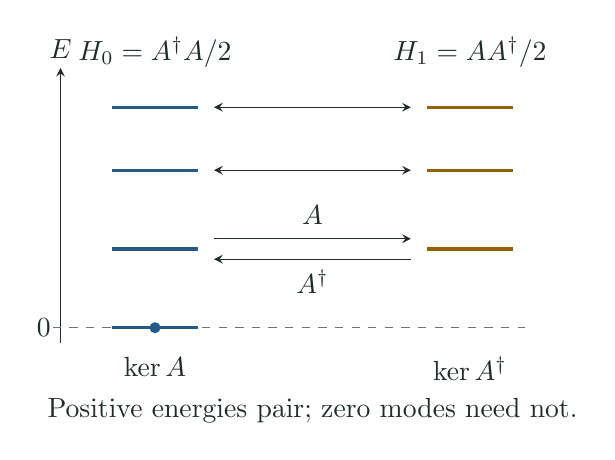
\begin{tikzpicture}[color=FigureForeground,>=stealth,x=1cm,y=1cm]
\draw[->] (-1.2,-.2)--(-1.2,3.3) node[above] {$E$};
\node at (0,3.5) {$H_0=A^\dagger A/2$};
\node at (4,3.5) {$H_1=AA^\dagger/2$};
\foreach \y in {1,2,2.8}{
 \draw[FigureBlue,very thick] (-.55,\y)--(.55,\y);
 \draw[FigureOrange,very thick] (3.45,\y)--(4.55,\y);
 \ifdim\y pt>1pt \draw[<->] (.75,\y)--(3.25,\y); \fi
}
\draw[->] (.75,1.13)--(3.25,1.13);
\draw[<-] (.75,.87)--(3.25,.87);
\node at (2,1.43) {$A$};
\node at (2,.58) {$A^\dagger$};
\draw[dashed,FigureMuted] (-1.3,0)--(4.7,0);
\node[left] at (-1.2,0) {$0$};
\draw[FigureBlue,very thick] (-.55,0)--(.55,0);
\fill[FigureBlue] (0,0) circle (2pt);
\node[below] at (0,-.25) {$\ker A$};
\node[below] at (4,-.25) {$\ker A^\dagger$};
\node at (2,-1.05) {\textnormal{Positive energies pair; zero modes need not.}};
\end{tikzpicture}
\end{document}
